\documentclass[11pt,fullpage]{article}
\usepackage{color, soul}
\usepackage{multicol,amsmath,amssymb,algorithmic}
\usepackage{graphics,graphicx}
\usepackage[right = 2.5cm, left=2.5cm, top = 2.5cm, bottom =2.5cm]{geometry}
\pagestyle{plain}
\def\urlfont{\DeclareFontFamily{OT1}{cmtt}{\hyphenchar\font='057}
              \normalfont\ttfamily \hyphenpenalty=10000}

%\input macros

\newcommand{\subheading}[1]{\noindent \textbf{#1}}
\newcommand{\grad}{\nabla}
\newcommand{\jump}[1]{[#1]}
\newcommand{\limit}[2]{\lim_{#1 \rightarrow #2}}
\newcommand{\mb}[1]{\mathbf{#1}}
\newcommand{\reals}[1]{\mathbb{R}^{#1}}
\newcommand{\blue}[1]{{\color{blue}{{#1}}}}

\title{Peridynamics-Based Fracture Animation for Elastoplastic Solids:\\
      Supplementary Technical Document}

\begin{document}
\maketitle

\section{Introduction}

This document presents the derivation of the constitutive model proposed in the paper. Section \blue{\ref{section:2}} introduces some preliminaries for the derivation and explains why the classical continuum elasticity theory could be regarded as a special case of peridynamics. Section \blue{\ref{section:3}} lists the common procedures to derive the peridynamics formulation of a general hyperelastic constitutive model in continuum mechanics. Finally, section \blue{\ref{section:4}} presents the derivation of the model introduced in the paper, which is a \emph{nonlocal} extension of the linear elastic model in the \emph{local} theory.

\section{Preliminaries}\label{section:2}

\subsection{Peridynamics equations of motion and the discretization}

As is introduced in the paper, in peridynamics the governing equation for any material point located at $\mb{x}$ is formulated as below:
\begin{equation}
\rho\ddot{\mb{u}}(\mb{x}) = \int_{H_\mb{x}}[\mb{T}<\mb{x}'-\mb{x}> - \mb{T}<\mb{x}-\mb{x}'>]dV_{\mb{x}}+\mb{b}(\mb{x}).
\label{eq:1}
\end{equation}
The state of material point at $\mb{x}$ is influenced by the possibly infinite number of material points $\mb{x}'$ that belong to its family $H_\mb{x}$. When the continuum is discretized into particles, the integral in Equation \blue{\ref{eq:1}} is replaced with the summations of particles within the horizon $\delta_\mb{x}$:
\begin{equation}
\rho\ddot{\mb{u}}(\mb{x}) = \sum_{\mb{x}',\mb{x}'\in H_\mb{x}}[\mb{T}<\mb{x}'-\mb{x}> - \mb{T}<\mb{x}-\mb{x}'>]V_{\mb{x}'}+\mb{b}(\mb{x}),
\label{eq:2}
\end{equation}
where $V_{\mb{x}'}$ is the volume of the discrete particle and its value depends on the distribution of particles.
\subsection{Peridynamics for local interactions}

In the limiting case where the horizon $\delta_\mb{x}$ approaches 0, the material point $\mb{x}$ interacts only with its immediate neighbors. See Figure \blue{\ref{fig:1}}, the material point with label $k$ interacts with the other six material points in the immediate vicinity denoted as $(k-l)$,$(k+l)$,$(k-m)$,$(k+m)$,$(k-n)$,and $(k+n)$. This conforms to the classical continuum mechanics, see the book \blue{\cite{bonet2008nonlinear}} for reference.
\begin{figure}[h]
  \centering
  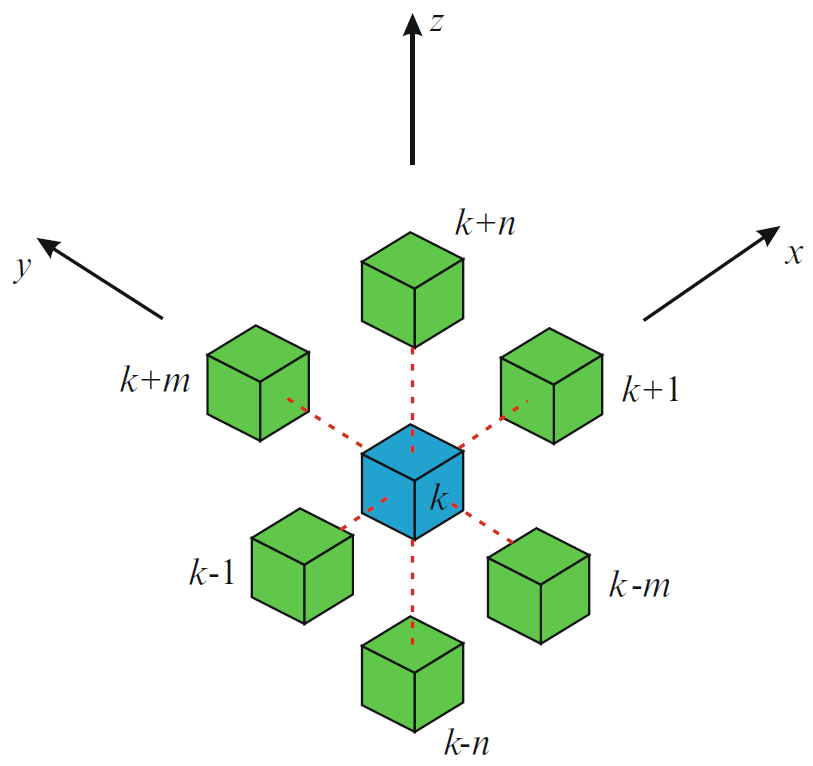
\includegraphics[width=0.5\linewidth]{./fig1.png}
  \caption{\label{fig:1}
  Material point $k$ interacts with its immediate neighborhood. Image from \blue{\cite{madenci2014peridynamic}}.
}
\end{figure}

In the context of local interactions, Equation \blue{\ref{eq:2}} for material point $k$ is represented in the following form:
\begin{equation}
\rho_{(k)}\ddot{\mb{u}}_{(k)} = \sum_{j=k-l,k+l,k-m,k+m,k-n,k+n}(\mb{t}_{(k)(j)}-\mb{t}_{(j)(k)})V_{(j)} + \mb{b}_{(k)},
\label{eq:3}
\end{equation}
where $\mb{t}_{(k)(j)}$ denotes the internal force density that material point $j$ exerted on point $k$, and $\mb{t}_{(j)(k)}$ is the other way around.

\subsection{Strain energy density and internal force density}

\section{Derivation for general hyperelastic materials}\label{section:3}

\section{Derivation for linear elastic materials}\label{section:4}

\bibliographystyle{eg-alpha}
\bibliography{../references}

\end{document}
